\cfoot{Samuel Schober}
Die Teamstruktur besteht aus dem Projekt Partner Ponix Systems, dem Betreuer, dem Product Owner sowie den Teammitgliedern. Für technische Betreuung sind der Projekt Partner sowie der Projekt Betreuer zuständig. Der Product Owner vertritt hierbei das Projekt nach außen und organisiert die Terminvereinbarungen zwischen dem Projekt Partner und dem Team.

\mbox{} \\ Das Projektteam setzt sich aus vier Mitgliedern zusammen. Jedes Teammitglied hat einen Aufgabenbereich zugewiesen, indem es die Hauptverantwortung trägt. Offizieller Teamleiter ist Samuel Schober. Er war vor allem beim Aufbau des Prototypen maßgeblich beteiligt und diente als Kontaktstelle zur Firma Ponix Systems. Als Stellvertretender Product Owner hat Matthias Schwebler im Laufe der Zeit auch die Koordination und die Abstimmung der einzelnen Bereiche übernommen. Die Bereiche der Sensordatenerfassung und -verarbeitung und die Aktorensteuerung waren seine Hauptaufgabenbereiche. Konrad Kelc betreute vor allem die Bereiche der Datenrecherche und der Datenarchivierung, während Ramin Bahadoorifar für die Erstellung der \gls{Webapp} und der Anbindung an das Backend übernahm. Eine detailierte Darstellung der Aufgabenteilung erfolgt im nächsten Kapitel. Zusätzlich ist zwecks besserer Übersichtlichkeit der Name des jeweiligen Verantwortlichen, sowie dessen Autor in der Fußzeile festgehalten.

\mbox{}\\In Abbildung 4 wird die Teamstruktur visualisiert:
\newpage

\begin{figure}[ht]
    \centering
	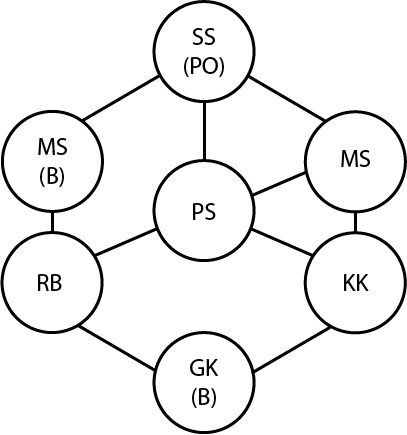
\includegraphics[width=8cm]{images/Teamstruktur_UrbanGreen}
    \caption{Teamstruktur}
\end{figure}\mbox{}\\

\textbf{Legende}
\begin{itemize}[leftmargin=4.5mm]
    \item{SS (PO):} Product Owner und Projektmitglied, Samuel Schober
    \item{MS (B):} Projektbetreuer, Markus Schabel
    \item{MS (POS):}  Product Owner Stellvertreter und Projektmitglied, Matthias Schwebler
    \item{PS:} Projektpartner, Ponix Systems
    \item{RB:} Projektmitglied, Ramin Bahadoorifar
    \item{KK:} Projektmitglied, Konrad Kelc
    \item{GK (B):} Projektbetreuer, Gottfried Koppensteiner
\end{itemize}

\newpage